\documentclass[a4paper,11pt,titlepage]{report}
\usepackage[printonlyused]{acronym}
\usepackage{amsmath}
\usepackage[UKenglish]{babel}
\usepackage{caption}
\usepackage{color}
\usepackage[hidelinks]{hyperref}
\usepackage{graphicx}
\usepackage[T1]{fontenc}
\usepackage[utf8]{inputenc}
\usepackage{listings}
\usepackage{lmodern}
\usepackage{url}

\renewcommand{\texttt}[1]{%
  \begingroup
  \ttfamily
  \begingroup\lccode`~=`/\lowercase{\endgroup\def~}{/\discretionary{}{}{}}%
  \begingroup\lccode`~=`[\lowercase{\endgroup\def~}{[\discretionary{}{}{}}%
  \begingroup\lccode`~=`.\lowercase{\endgroup\def~}{.\discretionary{}{}{}}%
  \catcode`/=\active\catcode`[=\active\catcode`.=\active
  \scantokens{#1\noexpand}%
  \endgroup
}

\title{\textbf{Network Attachment Point (NAP)}}
\author{Sebastian Robitzsch <sebastian.robitzsch@interdigital.com>}

\begin{document}
\setcounter{secnumdepth}{3} %enumerate up to subsubsection (not paragraph)
\lstset{language=C++}   
\maketitle
\tableofcontents
\newpage
\begin{acronym}[TDMA]
	\acro{CID}{content identifer}
	\acro{CMC}{Co-incidental Multicast}
	\acro{cNAP}{client-side \acl{NAP}}
	\acro{eNAP}{extended \acl{NAP}}
	\acro{FD}{file descriptor}
	\acro{FQDN}{Full Qualified Domain Name}
	\acro{FID}{forwarding identifier}
	\acro{GW}{Gateway}
	\acro{HTTP}{Hypertext Transfer Protocol}
	\acro{ICMP}{Internet Control Message Protocol}
	\acro{ICN}{Information-centric Networking}
	\acro{KPI}{Key Performance Indicator}
	\acro{LTP}{Lightweight Transport Protocol}
	\acro{MITU}{Maximum \acl{ICN} Transmission Unit}
	\acro{MOLY}{Monitoring Library}
	\acro{MTU}{Maximum Transmission Unit}
	\acro{NACK}{Negative Acknowledgement}
	\acro{NAP}{Network Attachment Point}
	\acro{NID}{Node Identifier}
	\acro{POINT}{iP Over IcN - the betTer ip}
	\acro{rCID}{reverse \acl{CID}}
	\acro{RTT}{Round Trip Time}
	\acro{RV}{Rendezvous}
	\acro{SDN}{Software-defined Networking}
	\acro{SE}{Session End}
	\acro{SED}{Session Ended}
	\acro{SK}{Session Key}
	\acro{sNAP}{sever-side \acl{NAP}}
	\acro{STL}{Standard Template Library}
	\acro{TCP}{Transport Control Protocol}
	\acro{TM}{Topology Manager}
	\acro{UE}{User Equipment}
	\acro{URL}{Uniform Resource Locator}
	\acro{UTP}{Unreliable Transport Protocol}
	\acro{WE}{Window End}
	\acro{WED}{Window Ended}
	\acro{WU}{Window Update}
	\acro{WUD}{Window Updated}
\end{acronym}

\acresetall
%%%%%%%%%%%%%%%%%%%%%%%%%%%%%%%%%%%%%%%%%%%%%%%%%%%%%%%%%%%%%
%%%%%%%%%%%%%%%%%%%%%%%%%%%%%%%%%%%%%%%%%%%%%%%%%%%%%%%%%%%%%
% CHAPTER
%%%%%%%%%%%%%%%%%%%%%%%%%%%%%%%%%%%%%%%%%%%%%%%%%%%%%%%%%%%%%
%%%%%%%%%%%%%%%%%%%%%%%%%%%%%%%%%%%%%%%%%%%%%%%%%%%%%%%%%%%%%
\chapter{Introduction}\label{ch:Introduction}
This document should be seen as some sort of \ac{NAP} documentation to bridge the gap between the POINT deliverables \cite{POINT}, describing \ac{NAP} functionality from a system perspective, and the code documentation available through Doxygen \cite{Heesch}. 
%%%%%%%%%%%%%%%%%%%%%%%%%%%%%%%%%%%%%%%%%%%%%%%%%%%%%%%%%%%%%
% Section
%%%%%%%%%%%%%%%%%%%%%%%%%%%%%%%%%%%%%%%%%%%%%%%%%%%%%%%%%%%%%
\section{Installation and Configuration of IP Service Endpoints}
The compilation and installation of the \ac{NAP} has been tested on Debian-based Linux distributions, i.e.:

\begin{itemize}
	\item Debian 8, 9
	\item Ubuntu 14.x, 15.x, 16.x
	\item Voyage 0.10
\end{itemize}

The following platforms have been successfully tested:
\begin{itemize}
	\item x86 and x86\_64 desktop and server machines
	\item APU and APU2s from PC Engines with Voyage and Debian installed)
	\item Raspberry Pi B, B+ and 3 with Debian (Raspbian installed)
\end{itemize}

The following virtualisation frameworks were successfuly tested too:
\begin{itemize}
	\item VirtualBox on Windows, Linux and MacOS hosts
	\item VMware on Windows hosts
	\item KVM on Debian and Ubuntu hosts
	\item vSphere
\end{itemize}

All required libraries in order to successfully compile the \ac{NAP} are listed in the Blackadder-wide list of libraries. Simply install all of them before making the NAP:

\begin{lstlisting}
~$ sudo apt install $(cat ~/blackadder/apt-get.txt)
\end{lstlisting}

As indicated in the README.md file, the NAP comes with a GNU-complaint make file which does not require any further customisation. Simply invoke \texttt{make} and provide the number of available cores to the \texttt{-j} argument to speed up the compilation, e.g. \texttt{make -j2} (no space between \texttt{-j} and the number of cores available for compilation]). To install the resulting binary called \texttt{nap} as a system-wide program run \texttt{sudo make install}. This copies the \ac{NAP} binary to \texttt{/usr/bin} and creates the configuration file directory \texttt{/etc/nap} (if it does not exist yet) as well as a template configuration file directory, \texttt{/usr/share/doc/nap}. 

When running the \ac{NAP} binary, the required configuration files are all expected to be located in \texttt{/etc/nap}. When calling \texttt{sudo make install} the Makefile attempts to copy the template configuration files to \texttt{/etc/nap}. If the files already exist in the destination directory the user is prompted if they should be overwritten. Simply answer yes (\texttt{y} or no (\texttt{n}.

\subsection{Internet Connectivity through an ICN Gateway}\label{sec:Introduciton_ICNGW}
When configuring the \ac{NAP} as an ICN gateway towards the Internet the configuration file of the \ac{NAP} acting as an ICN gateway must receive the following routing prefix configuration must be set (see Section~\ref{sec:Introduction_Var_networkAddressNetmask} for more details):

\begin{lstlisting}
	networkAddress = "0.0.0.0";
	netmask = "0.0.0.0";
\end{lstlisting}

Furthermore, it is advisable to tell the ICN gateway the routing prefix which covers all routing prefixes configured in the ICN networks. This limits the number of packets the demux must process to the one which are targeted at IP endpoints attached to other \acp{NAP} (see Section~\ref{sec:Introduction_Var_icnGw}.

The IP gateway which provides Internet access must receive the same configuration as IP service endpoints which do not have the \ac{NAP} as their default gateway. Please see the next section how to configure them accordingly.

In addition to adding the ICN gateway routing prefix to the \ac{NAP} which acts as the gateway all \acp{NAP} which are supposed to provide Internet access to their IP endpoints must receive the following routing prefix entry in their list of available prefixes (see Section~\ref{sec:Introduction_Var_RoutingPrefixes}):

\begin{lstlisting}
networkAddress = "0.0.0.0";
netmask = "0.0.0.0";
\end{lstlisting}

\subsection{Configure IP Service Endpoints}
In case the IP service endpoint attached to the \ac{NAP} does not have the NAP as its default IP gateway (e.g. an IP gateway which is performing NAT or a web server which has two interfaces) the IP routing table must have an entry which basically says all traffic from IP endpoints attached to other \acp{NAP} must be sent to the \ac{NAP} to which the IP service endpoint is attached to. Assuming the routing prefix which covers all \acp{NAP} is \texttt{172.16.0.0/16} and the \ac{NAP} the IP service endpoint is attached to has the IP address 172.16.123.1 the following rule must be inserted into the IP routing table:

\begin{lstlisting}
~$ route add -net 172.16.0.0 netmask 255.255.0.0 gw 172.16.123.1
\end{lstlisting}

Make sure that the interface which connects an IP service endpoint with its \ac{NAP} has a subnet which does not cover any other IP endpoint attached to another \ac{NAP}; this ensures that the configured gateway is always used for any communication and the IP service endpoint does not assume the IP endpoint is reachable within its subnet (this would cause ARP requests for the IP address which will remain unanswered).
%%%%%%%%%%%%%%%%%%%%%%%%%%%%%%%%%%%%%%%%%%%%%%%%%%%%%%%%%%%%%
% Section
%%%%%%%%%%%%%%%%%%%%%%%%%%%%%%%%%%%%%%%%%%%%%%%%%%%%%%%%%%%%%
\section{Configuration Variables}
This section explains the variables of the \ac{NAP}'s libconfig-based configuration file. The variables are listed in alphabetical ordered but can be placed in the configuration file in arbitrary order. All commented variables in the template nap.cfg file have the default value assigned to them so that the inexperienced user does not have to walk through the source code to find out which variable has been assigned with which default value.

\subsection{\texttt{bufferCleanerInterval}}\label{sec:Introduction_Var_BufferCleanerInterval}
All handlers have a buffer in case a packet cannot be published under its \ac{CID} due to various reasons (e.g. outstanding Blackadder notifications for this particular \ac{CID} such as START\_PUBLISH or START\_PUBLISH\_iSUB). The given value assigned to the variable determines the interval in seconds in which the buffer cleaner wakes up and checks all \ac{ICN} buffer cleaners for packets older than the interval the cleaner wakes up.

\subsection{\texttt{fqdns}}
\begin{itemize}
	\item[\texttt{fqdn}]: String, mandatory
	\item[\texttt{ipAddress}]: String, mandatory
	\item[\texttt{port}]: Integer, optional
\end{itemize}

\subsection{\texttt{interface}}\label{sec:Introduction_Var_interface}
This variable tells the \ac{NAP} on which local network device it communicates with IP endpoints. The argument to this variable must be given as a string and the interface name provided must have the IP assigned all the NAP's IP endpoints send their IP traffic to. Reason being how the NAP utilises PCAP, i.e. reading the host IP address to compile a PCAP filter which ignores packets sent directly to the NAP.

\subsection{\texttt{icnGwNetworkAddress} and \texttt{icnGwNetmask}}\label{sec:Introduction_Var_icnGw}
TODO More information about how to set up the \ac{NAP} as an ICN \ac{GW} is explained in Section~\ref{sec:Introduciton_ICNGW}.

\subsection{\texttt{ipEndpoint}}
For host-based deployments where the \ac{NAP} servers a single IP endpoint only the following variable must be uncommented and the IP address of the IP endpoint the NAP servers is stated there. The value must be given as a string.

\subsection{\texttt{ltpInitialCredit}}\label{sec:Introduction_Var_ltpInitialCredit}
The lightweight transport protocol for \ac{HTTP} packet delivery is using a credit-based transport mechanism, similar to SPDY/HTTP2. 

\subsection{\texttt{ltpRttListSize}}\label{sec:Introduction_Var_ltpRttListSize}
For obtaining the \ac{RTT} for \ac{LTP} timeout checkers the \ac{NAP} keeps a list of measured \ac{RTT} values to cope with potential \ac{RTT} outlier values. This variable allows to configure the size of the list which is used to obtain the average of all reported \ac{RTT} values.

\subsection{\texttt{ltpRttMultiplier}}\label{sec:Introduction_Var_ltpRttMultiplier}
As explained in further detail in Section~\ref{sec:Transport_LTP_RTT}, whenever \ac{LTP} starts a timeout counter to wait for a response from one of its receivers it uses a multiple of the previously measured \ac{RTT}. This particular multiplier can be changed with the variable \texttt{ltpRttMultiplier} which accepts unsigned integer values.

\subsection{\texttt{localSurrogateFqdn} and \texttt{localSurrogatePort}}\label{sec:Introduction_Var_localSurrogate}
In some scenarios a (static) surrogate is located on the same machine where the binary is running, i.e. localhost. In order to cope with this special use case two methods have been identified: 1) Using the kernel's ip routing table or 2) use the NAP to relay HTTP requests to an application running as a process on the same node. The two methods are described separately in the following two sections. Only Method 2 requires  \texttt{localSurrogateFqdn} to be set. Furthermore, variable \texttt{localSurrogatePort} allows to specify a port number different than 80 on which the IP service endpoint is listening on (only TCP sockets are supported). If \texttt{localSurrogatePort} is not given the \ac{NAP} assumes the IP service endpoint is listening on Port 80.

\subsubsection{Method: NAP}
If it is desired letting the \ac{NAP} process to handle \ac{HTTP} requests towards the local surrogate \texttt{localSurrogateMethod} must have value \texttt{nap}. Figure~\ref{fig:Local_Surrogacy_Method_NAP} illustrates the internals of this scenario. As can be seen, there are three physical interfaces present, i.e., eth0, eth1 and eth2. While eth0 is solely used to manage this node and eth1 to talk ICN, eth2 is facing the IP endpoints the \ac{NAP} is supposed to handle. Furthermore, the IP routing table of the kernel is illustrated along with the iptables entry to capture \ac{HTTP} requests targeted at destination IP addresses outside of the IP endpoints' subnet, i.e. 172.16.42.0/24 in this case. The iptables rule basically says that all TCP packets towards destination Port 80 (\ac{HTTP}) is forwarded to Port 3127 where the \ac{NAP}'s transparent \ac{HTTP} proxy is listening on (see the comment in the \ac{NAP}'s light blue box).
 
\begin{figure}[!htb]
	\centering
	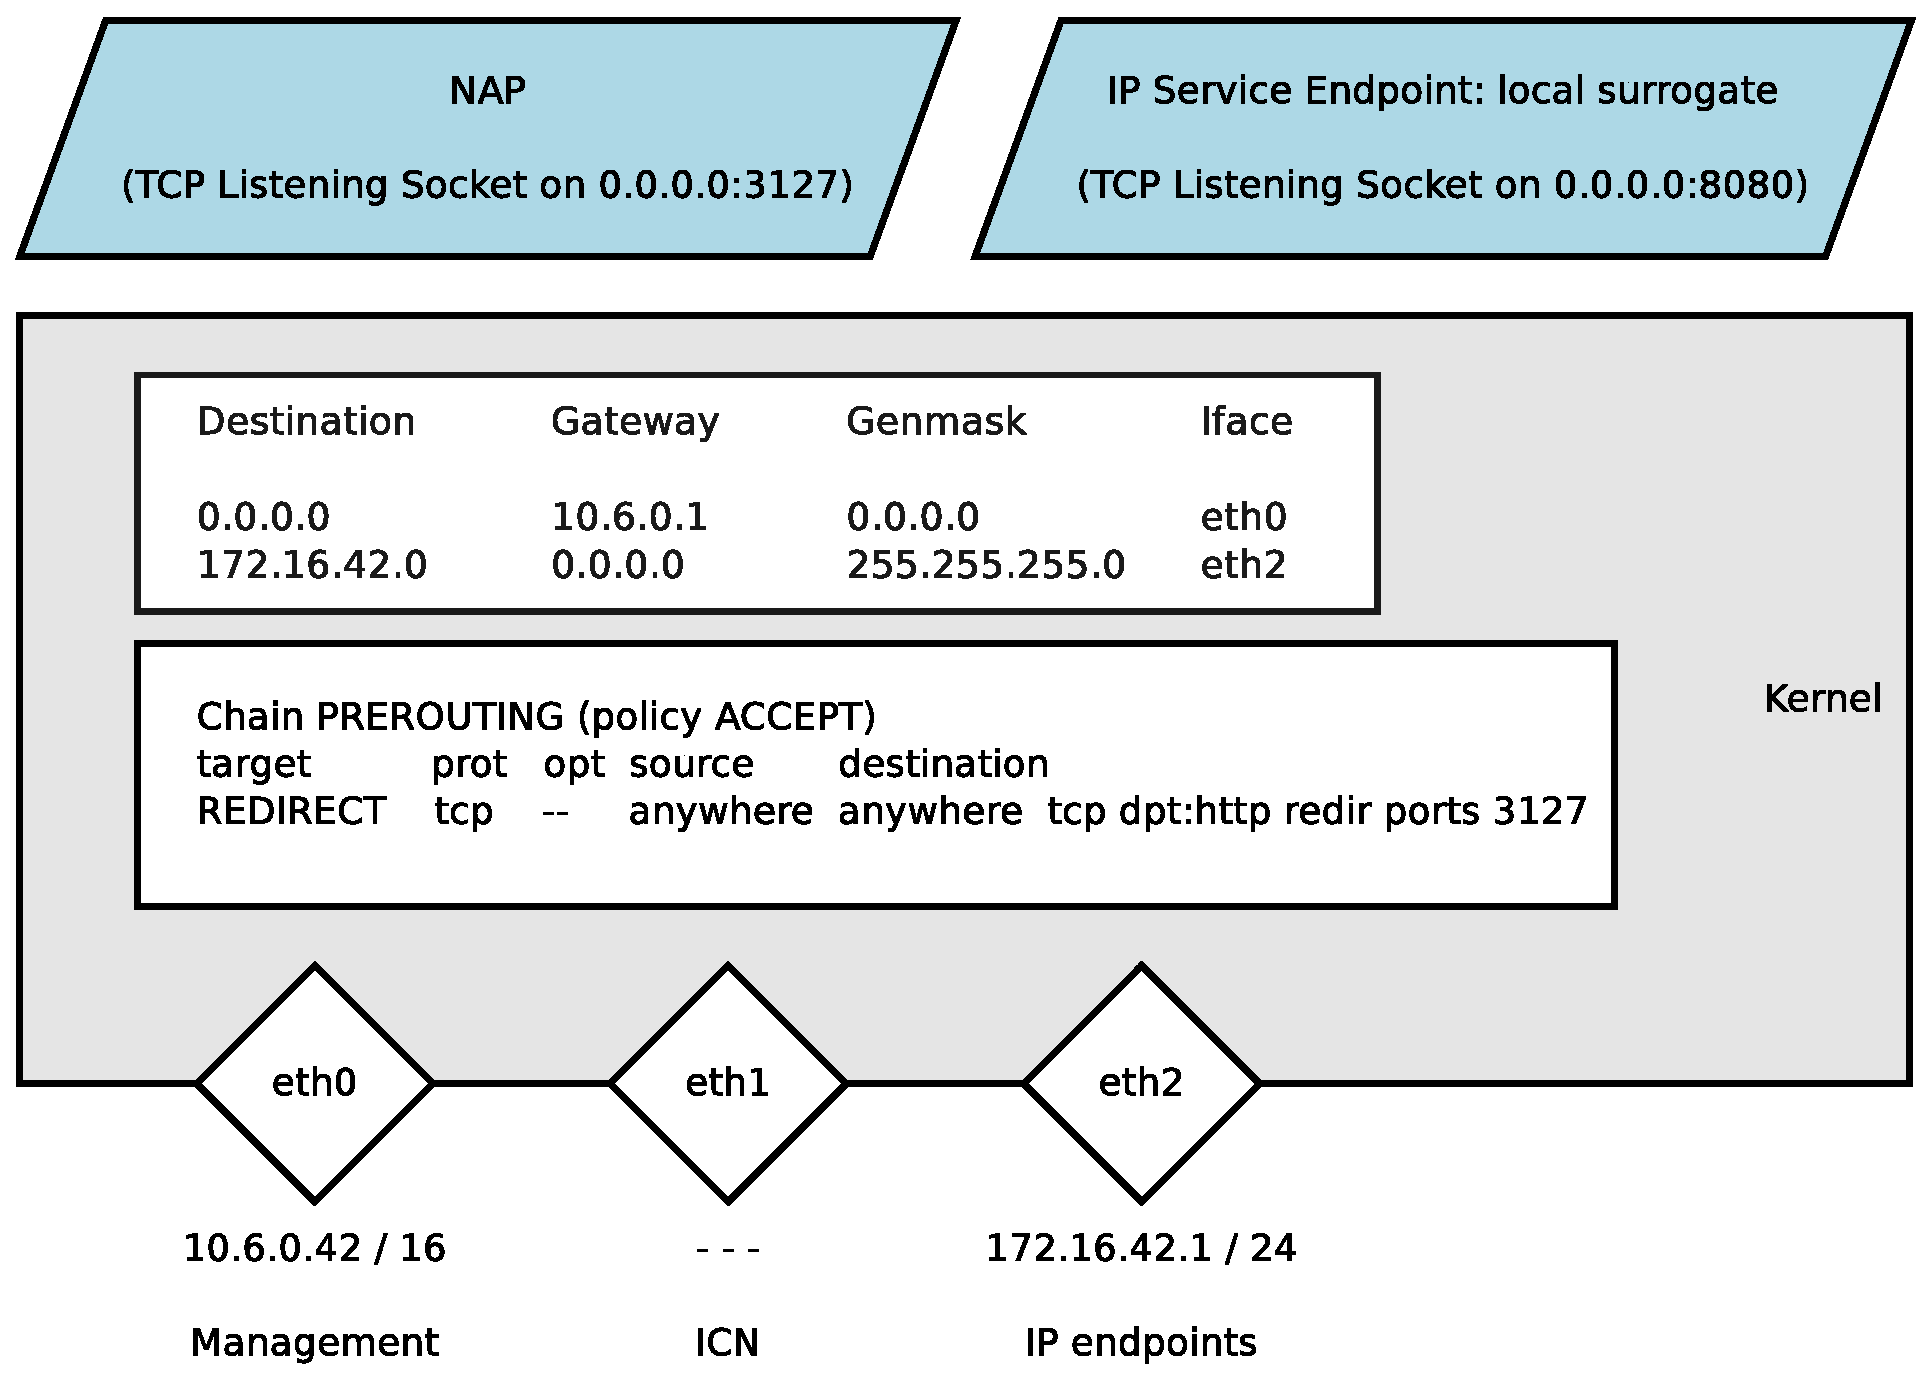
\includegraphics[width=1\linewidth]{eps/localSurrogacy-methodNap}
	\caption{Local surrogacy handled by the \acl{NAP}}
	\label{fig:Local_Surrogacy_Method_NAP}
\end{figure}

Any \ac{HTTP} request which arrives in the transparent proxy targeted at the \ac{FQDN} provided in \texttt{localSurrogateFqdn} is sent to the local surrogate via a TCP socket towards 127.0.0.1:8080 (assuming \texttt{localSurrogatePort = 8080}). Note that in scenarios where the IP service endpoint issues an \ac{HTTP} request to a port other than 80 is not supported by this implementation. In those scenario the kernel method is required, as described in the next section.

\subsubsection{Method: Kernel}
The other method to enable local surrogacy is using the kernel's IP routing table to forward an incoming packet towards an particular destination IP address outside the IP endpoints' subnet (172.16.42.0/24). This can be achieved by using iptables and and a PREROUTING policy which passes all TCP packets to the destination IP address 10.253.254.254 to the application on the same machine which is listening on Port 8080:

\begin{lstlisting}
~$ iptables -t nat -A PREROUTING -p tcp -d \
   10.253.254.254 -j REDIRECT --to-port 8080
\end{lstlisting}

\begin{figure}[!htb]
	\centering
	\includegraphics[width=1\linewidth]{eps/localSurrogacy-methodKernel}
	\caption{Local surrogacy directly handled by the kernel's IP routing table}
	\label{fig:Local_Surrogacy_Method_Kernel}
\end{figure}

The resulting iptables for this scenario and the overall set-up is illustrated in Figure~\ref{fig:Local_Surrogacy_Method_Kernel} which is identical to Figure~\ref{fig:Local_Surrogacy_Method_NAP} but a slightly different iptables configuration. So if an IP endpoint is issuing an \ac{HTTP} request to 10.253.254.254 the kernel of where the \ac{NAP} is running will forward this \ac{TCP} packet to the local surrogate which has a \ac{TCP} listener opened on Port 8080. Any \ac{HTTP} request to destination IP addresses other than 10.253.254.254 will be forwarded to the \ac{NAP}'s transparent \ac{HTTP} proxy which is listening on Port 3127.

\subsection{\texttt{httpHandler}}\label{sec:Introduction_Var_httpHandler}
In certain scenarios it is desired to not use the HTTP namespace for HTTP-level services. This can range from insufficient service level agreements to technical issues with particular HTTP services and the \ac{NAP} being incapable to translate them properly into the namespace; or the content/service provider simply does not want to enable this enhancement. For those cases the \ac{HTTP} handler can be turned off so that packets towards TCP Port 80 will not be mapped to the \ac{HTTP} namespace anymore. Consequently, all traffic will be treated as pure IP and the IP-over-ICN namespace will be used. The respective variable \texttt{httpHandler} allows the boolean values \texttt{true} and \texttt{false} which turns the \ac{HTTP} handler on and off, respectively.

\subsection{\texttt{httpProxyPort}}\label{sec:Introduction_Var_httpProxyPort}
For any HTTP traffic sent over TCP/IP with TCP destination Port 80 the \ac{NAP} handles the traffic differently leveraging the HTTP-over-ICN namespace. As the \ac{NAP} acts as a transparent proxy, a special iptables rule is inserted which forwards HTTP traffic to a port usually used by Squid.

\subsection{\texttt{mitu}}\label{sec:Introduction_Var_mitu}
This setting allows to lower the size of the \acl{MITU} the NAP publishes to the local ICN core. Reason being scenarios where VPNs or commercial links such as PPPoE are used as the underlying technology which require smaller Ethernet frames in order to not cause fragmentation. Adjusting the MITU accordingly can significantly boosts the performance of the NAP.

For more information about \ac{MITU} go to Section~\ref{sec:Code_Demux_Mitu}

\subsection{\texttt{molyInterval}}
The reporting of monitoring data points to the monitoring server is realised via \ac{MOLY}, a library available through Blackadder. The interval of how often available data points are being sent off is up to the process (in this case the \ac{NAP}). This interval can be configured here in seconds. The value given must be an integer. If the variable is not set or set to \texttt{0} the reporting to the monitoring agent is disabled. However, the \ac{NAP} still calls the corresponding class to collect monitoring data from across \ac{NAP} classes. More on this in Section~\ref{sec:Code_MOLY} on Page~\pageref{sec:Code_MOLY}.

\subsection{\texttt{networkAddress} and \texttt{netmask}}\label{sec:Introduction_Var_networkAddressNetmask}
Each \ac{NAP} acts in a particular routing prefix following the IP-over-ICN namespace definition. This routing prefix is configured here using a network address and a netmask. Both values must be given as a string. 

If the \ac{NAP} acts as an ICN \ac{GW} the both variables must receive the following values:

\begin{lstlisting}
	networkAddress = "0.0.0.0";
	netmask = "0.0.0.0";
\end{lstlisting}

Furthermore, it is advisable to manually configure the routing prefix the ICN GW is running on the interface towards the IP \ac{GW} which provides access to the Internet. Please see Section~\ref{sec:Introduction_Var_icnGw}.

\subsection{\texttt{routingPrefixes}}\label{sec:Introduction_Var_RoutingPrefixes}
The routing prefixes available in within the \ac{ICN} network can be configured using a list of pairs of \texttt{networkAddress} and \texttt{netmask}. As indicated in the example configuration file, both values must be provided as strings in a human readable format. The order of the prefixes does not matter, as the \ac{NAP} will order them according to their size (as in how many hosts a particular prefix comprises).

\subsection{\texttt{socketType}}\label{sec:Introduction_Var_SocketType}
First off, this option is not meant to be used unless there are issues with sent IP packets towards IP endpoints, i.e. they can be seen on the wire (with Tshark or TCPDUMP) but the endpoint does not reply or the NAP log states they have been sent off but nothing is seen on the wire. To date it seems that some Linux kernel/OS versions do not accept IP packets sent through a \texttt{IPPROTO\_RAW} socket. To mitigate this problem, the NAP can switch to Libnet \cite{Libnet} as an alternative to raw Linux IP sockets. If \texttt{socketType} is not set or commented the NAP uses the raw IP socket implementation of Linux to send Ip packets to endpoints.

\subsection{\texttt{tcpClientSocketBufferSize}}\label{sec:Introduction_Var_tcpClientSocketBufferSize}
The \ac{sNAP} (its transparent HTTP proxy to be precise) handles HTTP communications towards servers and is responsible to create, maintain and close TCP sockets towards the server; hence, the \ac{sNAP} acts as a TCP client towards the web server. This variable allows to configure the buffer size used when creating a TCP socket.

\subsection{\texttt{tcpInterceptionPort}}\label{sec:Introduction_Var_tcpInterceptionPort}
Configure the port on which the transparent HTTP proxy should intercept.

\subsection{\texttt{tcpServerSocketBufferSize}}\label{sec:Introduction_Var_tcpServerSocketBufferSize}

Note, for the time being the \ac{cNAP} does not perform flow control operations using \ac{LTP}'s \ac{WU} and \ac{WUD} control messages. Hence, the \ac{TCP} server packet buffer must be equal or smaller than the \ac{LTP} credit so that the \ac{cNAP} never requires to enforce \ac{LTP} flow control. The server socket buffer size can be easily calculated by
%
\begin{eqnarray}
\text{LTP}_{credit} * \text{MITU} \le \text{BufSize}\label{eq:TCP_SERVER_SOCKET_BUFFER_SIZE}
\end{eqnarray}

%%%%%%%%%%%%%%%%%%%%%%%%%%%%%%%%%%%%%%%%%%%%%%%%%%%%%%%%%%%%%
% Section
%%%%%%%%%%%%%%%%%%%%%%%%%%%%%%%%%%%%%%%%%%%%%%%%%%%%%%%%%%%%%
\section{Logging and Debugging}\label{sec:Introduction_Logging}
The \ac{NAP} utilises Apache's log4cxx logging library which allows a class-based logging combined with a highly customisable output formats. When installing the \ac{NAP} a default log4cxx configuration file, nap.l4j, is placed in \texttt{/etc/nap} which has all available classes set to logging level \texttt{INFO}. The following logging levels are used in the \ac{NAP}:
\begin{itemize}
	\item[\texttt{ERROR}:] A crucial error within the \ac{NAP} which causes malfunction behaviour and/or a complete stop/crash/hang of a particular \ac{NAP} functionality. If such an error occurs please double check your \ac{NAP} configuration file or consult the POINT community on github.
	\item[\texttt{WARN}:] An unexpected behaviour in the sequence of actions which causes the \ac{NAP} to not being able to process the message properly. 
	\item[\texttt{INFO}:] Important information about the start/stop of a \ac{NAP} module.
	\item[\texttt{DEBUG}:] Debugging information about a particular class which informs the user about the overall functional healthiness of the \ac{NAP} and the class where this logging level is set in particular.
	\item[\texttt{TRACE}:] A per packet status while it traverses the \ac{NAP}. Note, this can cause a sheer flood of logging messages. Please use with caution and enable only when debugging the \ac{NAP}'s internals.
\end{itemize}

The logging output can be configured to stdout and the filesystem using the \texttt{log4j.rootLogger} identifier. The default is set to both and the log file can be found in the default Linux log directory, i.e. \text{/var/log/nap.log}. The size and number of log files can be configured using the \texttt{log4j.appender.R} identifier. For more information on how to use log4cxx please consult Apache's documentation.
%%%%%%%%%%%%%%%%%%%%%%%%%%%%%%%%%%%%%%%%%%%%%%%%%%%%%%%%%%%%%
%%%%%%%%%%%%%%%%%%%%%%%%%%%%%%%%%%%%%%%%%%%%%%%%%%%%%%%%%%%%%
% CHAPTER
%%%%%%%%%%%%%%%%%%%%%%%%%%%%%%%%%%%%%%%%%%%%%%%%%%%%%%%%%%%%%
%%%%%%%%%%%%%%%%%%%%%%%%%%%%%%%%%%%%%%%%%%%%%%%%%%%%%%%%%%%%%
\chapter{ICN Namespaces}\label{ch:IcnNamespaces}
%%%%%%%%%%%%%%%%%%%%%%%%%%%%%%%%%%%%%%%%%%%%%%%%%%%%%%%%%%%%%
% Section
%%%%%%%%%%%%%%%%%%%%%%%%%%%%%%%%%%%%%%%%%%%%%%%%%%%%%%%%%%%%%
\section{IP}\label{sec:IcnNamespaces_IP}
The IP namespace and its implementation in the IP handler is the fallback for all traffic which is not handled by any other namespace.
%%%%%%%%%%%%%%%%%%%%%%%%%%%%%%%%%%%%%%%%%%%%%%%%%%%%%%%%%%%%%
% Section
%%%%%%%%%%%%%%%%%%%%%%%%%%%%%%%%%%%%%%%%%%%%%%%%%%%%%%%%%%%%%
\section{HTTP}\label{sec:IcnNamespaces_HTTP}
The HTTP namespace and its implementation in the HTTP handler applies to all traffic classified as HTTP, i.e. TCP towards Port 80 (unless specified otherwise in nap.cfg).
%%%%%%%%%%%%%%%%%%%%%%%%%%%%%%%%%%%%%%%%%%%%%%%%%%%%%%%%%%%%%
% Section
%%%%%%%%%%%%%%%%%%%%%%%%%%%%%%%%%%%%%%%%%%%%%%%%%%%%%%%%%%%%%
\section{IGMP}\label{sec:IcnNamespaces_IGMP}
The IGMP namespace and its implementation in the IGMP handler applies to all traffic classified as IGMP.
%%%%%%%%%%%%%%%%%%%%%%%%%%%%%%%%%%%%%%%%%%%%%%%%%%%%%%%%%%%%%
% Section
%%%%%%%%%%%%%%%%%%%%%%%%%%%%%%%%%%%%%%%%%%%%%%%%%%%%%%%%%%%%%
\section{Management}\label{sec:IcnNamespaces_Management}
\subsection{DNS Local}
The information item \texttt{DNSlocal} allows \acp{eNAP} to inform any other \ac{NAP} about a change in the number of publisher for a particular \ac{FQDN} under the \texttt{/http} namespace. As all \acp{FID} for \texttt{/http/fqdn} in \acp{cNAP} are only requested from RV/TM if they do not exist in the local ICN core, i.e. Blackadder, DNS local allows to trigger the flushing of \acp{FID} in the core locally for a particular \ac{FQDN}.
\subsection{Monitoring}
%%%%%%%%%%%%%%%%%%%%%%%%%%%%%%%%%%%%%%%%%%%%%%%%%%%%%%%%%%%%%
%%%%%%%%%%%%%%%%%%%%%%%%%%%%%%%%%%%%%%%%%%%%%%%%%%%%%%%%%%%%%
% CHAPTER
%%%%%%%%%%%%%%%%%%%%%%%%%%%%%%%%%%%%%%%%%%%%%%%%%%%%%%%%%%%%%
%%%%%%%%%%%%%%%%%%%%%%%%%%%%%%%%%%%%%%%%%%%%%%%%%%%%%%%%%%%%%
\chapter{Transport Protocols}
%%%%%%%%%%%%%%%%%%%%%%%%%%%%%%%%%%%%%%%%%%%%%%%%%%%%%%%%%%%%%
% Section
%%%%%%%%%%%%%%%%%%%%%%%%%%%%%%%%%%%%%%%%%%%%%%%%%%%%%%%%%%%%%
\section{\acl{UTP}}\label{sec:Transport_UTP}
The \ac{UTP} only serves a single purpose: fragmentation and stitching the packets back together at the other side. \ac{UTP} is plugged to the IP handler and fragments all packets which exceeds the maximum ac{ICN} payload. If the \ac{NAP} receives a packet larger than the \ac{MITU} the paket gets fragmented by the sending \ac{NAP} and put into an \ac{UTP} packet as payload. Each \ac{UTP} packet has a predefined header, as illustrated in Figure~\ref{fig:UnreliableTransportProtocol}. The definition of the fields is defined by \texttt{utp\_header\_t} defined in \texttt{transport/unreliabletypedef.hh}.

\begin{figure}[!htb]
	\centering
	\includegraphics[width=1\linewidth]{eps/utpPacketFormat}
	\caption{\ac{UTP} packet format}
	\label{fig:UnreliableTransportProtocol}
\end{figure}

\paragraph{Key} The key is generated by the sending \ac{NAP} and allows to differentiate between several \ac{UTP} sessions. The key is a sum of the hashed destination \ac{CID} and a random value generated by \texttt{rand()}. This can be found in the \texttt{Unreliable::publish()} method in \texttt{transport/unreliable.cc}.
\paragraph{Payload Length} This field indicates the length of the payload length followed after the \ac{UTP} header.
\paragraph{Sequence} This field indicates the position of the fragment for the packet reassembly after receiving all fragments. 
\paragraph{State} This field indicates if the packet is the first, an intermediate or the last one. In case the \ac{UTP} packet carries a single fragment only without any preceding or succeeding packet the state is set to "single" packet. The states are defined in the enumeration \texttt{TransportStates}.
\paragraph{Payload} The payload of the \ac{UTP} header carrying the IP packet.
%%%%%%%%%%%%%%%%%%%%%%%%%%%%%%%%%%%%%%%%%%%%%%%%%%%%%%%%%%%%%
% Section
%%%%%%%%%%%%%%%%%%%%%%%%%%%%%%%%%%%%%%%%%%%%%%%%%%%%%%%%%%%%%
\section{\acl{LTP}}\label{sec:Transport_LTP}
This section describes the cornerstones of the \ac{LTP} implementation. The design description of this protocol can be found in Deliverable 2.3 of the POINT project \cite{POINT-D2.3}.
\subsection{Header Format}
\subsubsection{Control Plane Header}
The \ac{LTP} packet header for control plane traffic is illustrated in Figure~\ref{fig:LTPPacketFormat-CTRL}. There are seven different \ac{LTP} control plane packets realised following the \ac{LTP} specification:

\begin{itemize}
	\item \ac{LTP}-\ac{NACK}
	\item \ac{LTP}-\ac{SE}
	\item \ac{LTP}-\ac{SED}
	\item \ac{LTP}-\ac{WE}
	\item \ac{LTP}-\ac{WED}
	\item \ac{LTP}-\ac{WU}
	\item \ac{LTP}-\ac{WUD}
\end{itemize}

\begin{figure}[ht]
	\begin{center}
		\includegraphics[width=0.5\textwidth]{eps/ltpPacketFormat-ctrl}
		\caption{\acl{LTP} control plane packet format}
		\label{fig:LTPPacketFormat-CTRL}
	\end{center}
\end{figure}

All \ac{LTP} control plane headers are implemented in \texttt{transport/lightweighttypedef.hh} as \texttt{struct} with \ac{LTP} message type and control type messages enumerated in \texttt{enumerations.hh} (\texttt{ltp\_message\_types\_t} and \texttt{ltp\_ctrl\_control\_types\_t}).

\subsubsection{Data Plane Header}
The \ac{LTP} header for data plane traffic is illustrated in Figure~\ref{fig:LTPPacketFormat-Data} and consists of the four fields:

\begin{itemize}
	\item \ac{LTP} Type: Using \texttt{LTP\_DATA} this field indicating that this \ac{LTP} message is a data plane packet. 
	\item Session Key: A per node unique integer identifying the HTTP session (derived from the socket file descriptor in the HTTP proxy)
	\item Sequence: A continuous sequence number indicating the position of the fragment
	\item Payload Length: The length of the \ac{LTP} payload field in octets
\end{itemize}

\begin{figure}[ht]
	\begin{center}
		\includegraphics[width=1\textwidth]{eps/ltpPacketFormat-data}
		\caption{\acl{LTP} data plane header format}
		\label{fig:LTPPacketFormat-Data}
	\end{center}
\end{figure}

\subsection{\acl{RTT}}\label{sec:Transport_LTP_RTT}
\ac{RTT} measurements are used as a timeout to discover that an \ac{LTP} control message was potentially lost and must be therefore resent in order to keep the state machines in all \acp{NAP} participating in the same \ac{LTP} session sychronised. The \ac{NAP} measures \ac{RTT} after finish publishing a full packet received from the IP endpoint by issuing an \ac{LTP} \ac{WE} packet and awaiting the corresponding response, i.e. \ac{WED}. This behaviour is realised in the public \texttt{Lightweight::publish()} methods (\texttt{transport/lightweight.*}), one for \ac{HTTP} requests with \ac{CID} and \ac{rCID} and one for \ac{HTTP} responses where the \ac{rCID} and a list of \acp{NID} is used. Both methods publish the data using \texttt{Lightweight::\_publishData()} and issue a \ac{WU} \ac{LTP} control message right after. This is followed by a time-based counter to check for the corresponding awaited \ac{WED} control message in order to proceed with the next packet from the IP endpoint. The time to wait is defined by a multiple of the currently known \ac{RTT}. This multiplier is a fixed value stored in a private member of class \texttt{Lightweight}, i.e. \texttt{\_timeout}.

To deal with measure \ac{RTT} values much larger or smaller then the currently known \ac{RTT} the \ac{NAP} has a list of previously obtained \acp{RTT} and calculates the mean over them every time a new \ac{LTP} session is created. This operation has been implemented in \texttt{Lightweight::\_rtt()} which uses a default list size of 10 values. The list size can be configured using \texttt{ltpRttListSize} in the \ac{NAP}'s configuration file (see Section~\ref{sec:Introduction_Var_ltpRttListSize}).

In order to accommodate for the possibility that a remote \ac{NAP} disappears during an on-going \ac{LTP} session the \ac{NAP} always gives up to check for a received \ac{WUD} after 23 attempts following the 23 enigma\footnote{\url{https://en.wikipedia.org/wiki/23_enigma}}.
%%%%%%%%%%%%%%%%%%%%%%%%%%%%%%%%%%%%%%%%%%%%%%%%%%%%%%%%%%%%%
%%%%%%%%%%%%%%%%%%%%%%%%%%%%%%%%%%%%%%%%%%%%%%%%%%%%%%%%%%%%%
% CHAPTER
%%%%%%%%%%%%%%%%%%%%%%%%%%%%%%%%%%%%%%%%%%%%%%%%%%%%%%%%%%%%%
%%%%%%%%%%%%%%%%%%%%%%%%%%%%%%%%%%%%%%%%%%%%%%%%%%%%%%%%%%%%%
\chapter{Code Structure and Implementation Design Choices}
\section{Demultiplexer}\label{sec:Code_Demux}
The implementation of demultiplexing incoming packets slightly differs from the \ac{NAP}'s architectural description. While the \ac{POINT} Deliverable 3.1 \cite{POINT-D3.1} illustrates a single functional box which receives packets from the IP endoint and determines which handler they belong to the implementation of the NAP uses two orthorgonal methods; one for HTTP-over-ICN traffic and one for the remaining packets. For HTTP-over-ICN packets an iptables rule is inserted to forward all traffic to a particular TCP port to another port where the NAP's HTTP proxy is listening on.

By default the TCP interception port for HTTP-over-ICN is set to TCP communications towards Port 80 which is forwarded to Port 3127, the very same port used by Squid for transparent proxy interceptions. If the HTTP service is using a server port other than 80 this can be configured in the NAP's configuration file (see Section~\ref{sec:Introduction_Var_tcpInterceptionPort} for more details). The NAP has its own transparent HTTP proxy which (transparently) listens on Port 3127 and terminates TCP session that arrive on this port with the help of the modified iptables. The modified iptables rules can be checked by invoking the following command after the \ac{cNAP} has been started:

\texttt{\$ iptables -L -t nat}

\subsection{\acl{MITU}}\label{sec:Code_Demux_Mitu}
The POINT platform places the ICN packet (ICN header + payload) straight in Layer 2 frames. Thus, what \ac{MTU} is for IP packets, the \ac{MITU} is for ICN packets. For IP-over-ICN scenarios where the entire IP packet (header + payload) is placed as payload to an ICN packet an ICN link which does not support jumbo frames will force the NAP to fragment packets with an \ac{MTU} + IP header larger than the \ac{MITU}. Hence, the NAP checks for every packet that is provisioned by PCAP if the length is larger than the \ac{MITU} which is configured in the NAP's configuration file\footnote{See Section~\ref{sec:Introduction_Var_mitu}}. In case the packet is handled in the IP-over-ICN handler the NAP follows RFC 792 \cite{rfc792} which states that if the Don't Fragment flag is set in the IP header the packet must not be fragmented and an \ac{ICMP} packet of Type 3, Code 4 must be issued to inform the sending IP endpoint to lower its \ac{MTU}.
%%%%%%%%%%%%%%%%%%%%%%%%%%%%%%%%%%%%%%%%%%%%%%%%%%%%%%%%%%%%%
% Section
%%%%%%%%%%%%%%%%%%%%%%%%%%%%%%%%%%%%%%%%%%%%%%%%%%%%%%%%%%%%%
\section{Types}
todo
\subsection{Eui48}\label{sec:Types_eui48}
\texttt{types/eui48.*}
\subsection{IcnId}\label{sec:Types_IcnId}
\texttt{types/icnid.*}
\subsection{IpAddress}\label{sec:Types_IpAddress}
\texttt{types/ipaddress.*}
\subsection{Netmask}\label{sec:Types_Netmask}
\texttt{types/netmask.*}
\subsection{NodeId}\label{sec:Types_NodeId}
\texttt{types/nodeid.*}
\subsection{RoutingPrefix}\label{sec:Types_RoutingPrefix}
\texttt{types/routingprefix.*}
%%%%%%%%%%%%%%%%%%%%%%%%%%%%%%%%%%%%%%%%%%%%%%%%%%%%%%%%%%%%%
% Section
%%%%%%%%%%%%%%%%%%%%%%%%%%%%%%%%%%%%%%%%%%%%%%%%%%%%%%%%%%%%%
\section{Transparent HTTP Proxy}\label{sec:Code_Transparent_HTTP_Proxy}
As HTTP-over-ICN is one of the key namespaces that bring several \ac{KPI} improvments to an operator's network, the handling of HTTP messages are discuss in more detail in this section. The HTTP proxy and the handling of TCP sockets is the main focus of this section.

\subsection{Handling HTTP Messages}
As mentioned several times already, the \ac{NAP} acts as a transparent \ac{HTTP} proxy by which \ac{TCP} sessions that carry \ac{HTTP} packets are terminated at the \ac{NAP} node. This termination is part of the HTTP proxy implementation which is located in \texttt{proxies/http}. The following sub-sections describe the handling of HTTP request and response messages in NAP (and the proxy in particular). 

Just for clarification: all \acp{NAP} can act as a \ac{cNAP} or \ac{sNAP}. It all depends on which IP endpoint issues an HTTP request and which one serves a paritcular \ac{FQDN} to label a \ac{NAP} as client- or server-side \ac{NAP}.

\subsubsection[cNAP Operations for HTTP Requests]{Client-side NAP Operations for HTTP Requests}
With the help of an appropriate \texttt{iptables} entry incoming \ac{TCP} packets towards a particular port\footnotetext{By default Port 80; the variable \texttt{tcpInterceptionPort} in nap.cfg allows to customise it. See Section~\ref{sec:Introduction_Var_tcpInterceptionPort} for more details} are routed to the port where the \ac{NAP} is listening\footnotetext{By default port 3127; the variable \texttt{httpProxyPort} in nap.cfg allows to customise it. See Section~\ref{sec:Introduction_Var_httpProxyPort} for more details}. The listening socket to accept \ac{TCP} sessions is created in the functor \texttt{HttpProxy::operator()} in \texttt{proxies/http/httpproxy.cc} and is illustrated at the top in Figure~\ref{fig:Handling_HTTP_requests_cNAP}. Upon the establishment of a new \ac{TCP} session the function \texttt{accept()} returns the new socket \ac{FD} which is then given to a new thread together with the IP address of the new endpoint. The functor \texttt{TcpServer::operator()} in \texttt{proxies/http/tcpserver.cc} then handles the accepted socket by reading the incoming packet.

\begin{figure}[!htb]
	\centering
	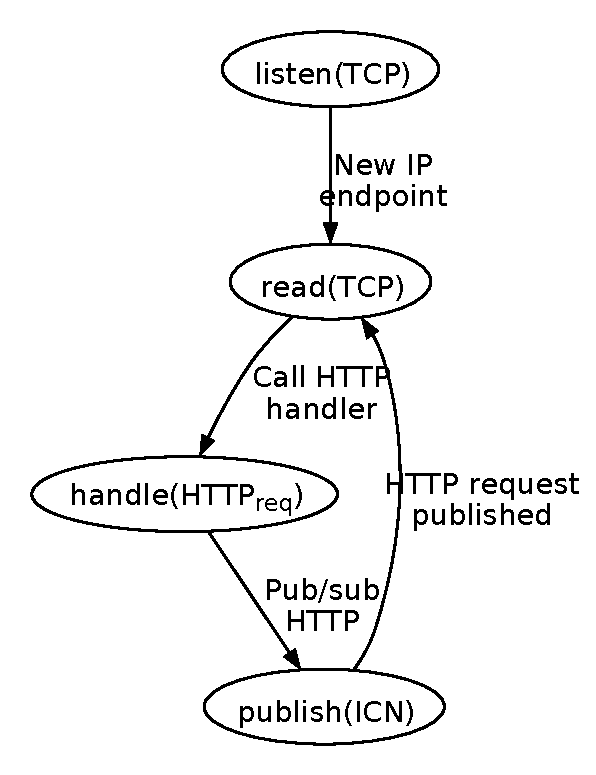
\includegraphics[width=0.5\linewidth]{eps/proxyStateMachine-HTTPrequests-cNAP}
	\caption{cNAP states when handling HTTP requests}
	\label{fig:Handling_HTTP_requests_cNAP}
\end{figure}

The \texttt{TcpServer} class then reads the \ac{FQDN}, \ac{HTTP} method and the web resource which allows the \ac{HTTP} proxy to determine whether this packet is a new \ac{HTTP} sessions or a continuation. If the \ac{HTTP} request is using method \texttt{POST} or \texttt{PUT} it is quite likely that a single \ac{HTTP} spans over several \ac{TCP} packets. Hence, the necessity of reading the three values from the \ac{HTTP} request and keeping state in the functor.

For every incoming \ac{HTTP} fragment the proxy calls the appropriate method of the \ac{HTTP} handler, i.e. \texttt{Http::handleRequest} in \texttt{namespaces/http.cc}. The \ac{HTTP} handler now determines whether the \ac{CID} \texttt{/http/fqdn} has been already published to the \ac{RV} or the information item \texttt{FQDN} is unknown to the \ac{NAP}. If it is the latter, the information item \texttt{/fqdn} is published under the scope path \texttt{/http} and the \ac{HTTP} packet/fragment is added to the proxy buffer\footnotetext{More information about the various packet buffers can be found in Section~\ref{sec:Code_NapPacketBuffers}}. If the \ac{CID} has been already published the \ac{HTTP} handler checks if a \texttt{START\_PUBLISH} notification had been received from the local ICN core indicating that the \ac{RV} has matches at least one subscriber to \texttt{/http/fqdn} (i.e. an \ac{sNAP}) and the \ac{TM} has provided a \ac{FID} for the path. Assuming the \ac{FID} is available the \ac{HTTP} handler passes the packet over to \ac{LTP} to eventually publishes the packet.

\subsubsection[sNAP Operations for HTTP Requests]{Server-side NAP Operations for HTTP Requests}
The \ac{NAP} continuously listens for new incoming data and control plane ICN packets using the non-blocking Blackadder API method \texttt{Blackadder::getEvent} located in \texttt{icncore/icn.cc}. If an HTTP request fragment has been received the Blackadder event identifier \texttt{PUBLISH\_DATA\_iSUB} is used and if the \ac{LTP} transaction has successfully finished the state \texttt{TP\_STATE\_ALL\_FRAGMENTS\_RECEIVED} is returned from \texttt{Transport::handle()} indicating that the \ac{HTTP} packet can be handed over to the proxy. This is achieved through the \texttt{TcpClient::operator()} functor, located in \texttt{proxies/http/tcpclient.cc}, which is called from within the ICN core handler in order to be placed into a thread.

\begin{figure}[!htb]
	\centering
	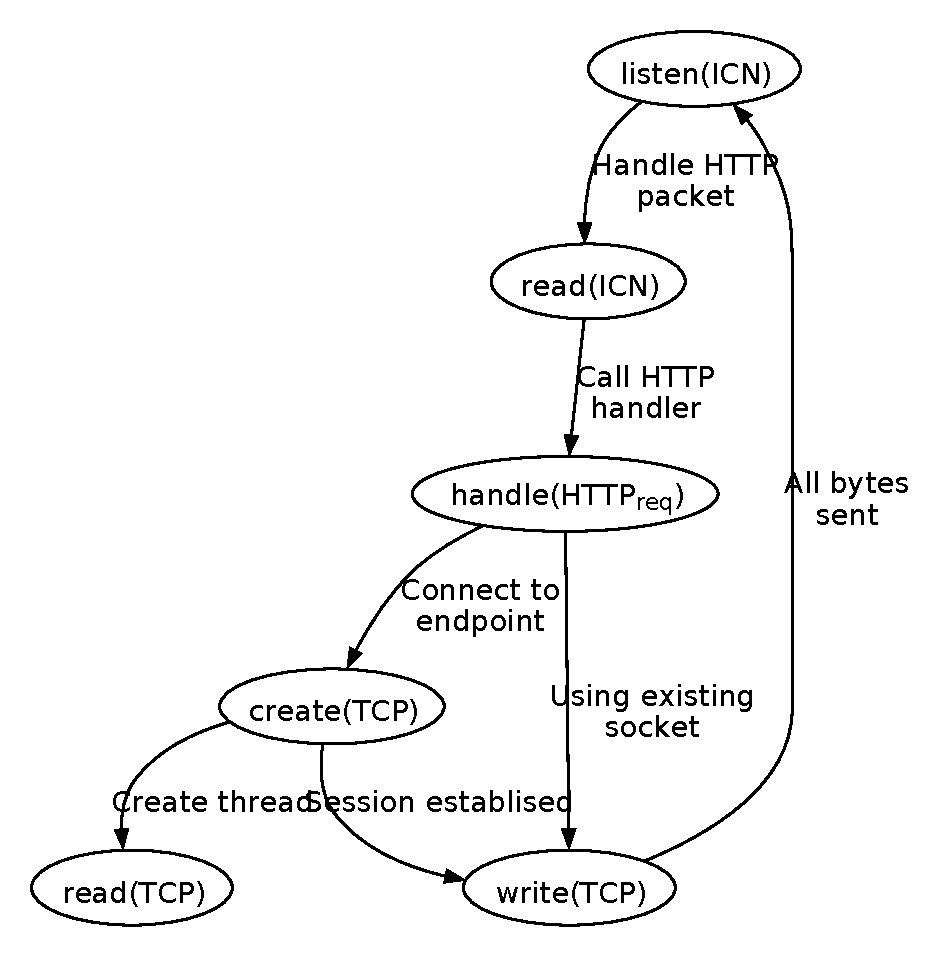
\includegraphics[width=0.8\linewidth]{eps/proxyStateMachine-HTTPrequests-sNAP}
	\caption{sNAP states when handling HTTP requests}
	\label{fig:Handling_HTTP_requests_sNAP}
\end{figure}

As illustrated in Figure~\ref{fig:Handling_HTTP_requests_sNAP} in the bottom left corner, the \ac{HTTP} proxy determines whether a new socket is to be created or an existing \ac{FD} can be used. In case a new socket is created (\texttt{TcpClient::\_tcpSocket()} in \texttt{proxies/http/tcpclient.cc}) the \texttt{read()} function is called in a thread using the \texttt{TcpClientThread::operator()} functor located in \texttt{proxies/http/tcpclientthread.cc}. Note, the reason why the reading thread is created before the writing to the socket takes place is due to an observation when conducting trials. In NAP releases lower than 3.2.1 \texttt{read()} was called in the same thread where \texttt{write()} took place and under heavy load the \ac{sNAP} was not able to complete all the steps in between on time (writing states to internal maps) which caused a \texttt{SIGPIPE} event and the end of the \ac{sNAP} process.\footnotetext{\url{https://www.gnu.org/software/libc/manual/html\_mono/libc.html\#Operation-Error-Signals}, "You have to design your application so that one process opens the pipe for reading before another starts writing."}

\subsubsection{\acl{sNAP} Operations for HTTP Responses}
\begin{figure}[!htb]
	\centering
	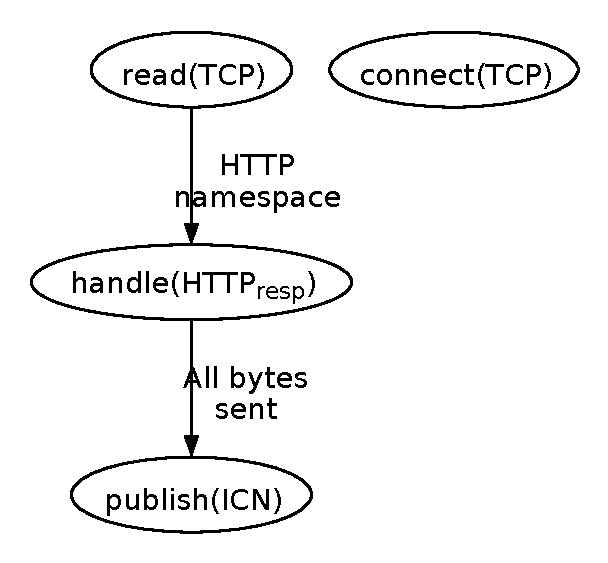
\includegraphics[width=1\linewidth]{eps/proxyStateMachine-HTTPresponses-sNAP}
	\caption{sNAP states when handling HTTP responses}
	\label{fig:Handling_HTTP_responses_sNAP}
\end{figure}
\subsubsection{\acl{cNAP} Operations for HTTP Responses}
\begin{figure}[!htb]
	\centering
	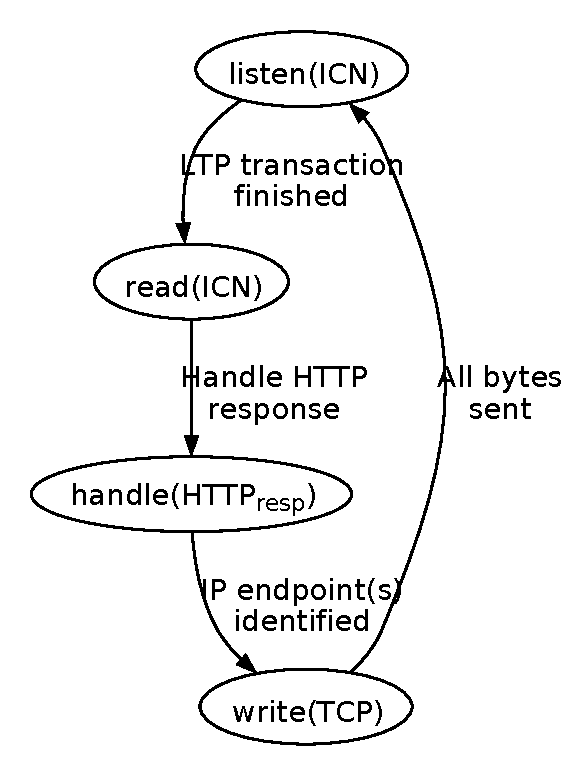
\includegraphics[width=1\linewidth]{eps/proxyStateMachine-HTTPresponses-cNAP}
	\caption{cNAP states when handling HTTP responses}
	\label{fig:Handling_HTTP_responses_cNAP}
\end{figure}

\subsection{TCP Socket Handling}
For \ac{HTTP}-level services using \ac{TCP} destination Port 80 the \ac{cNAP} intercepts the \ac{TCP} session and acts as a \ac{TCP} server, as described in further detail in Section~\ref{sec:Code_Transparent_HTTP_Proxy}. Consequently, the \ac{sNAP} acts as a \ac{TCP} client towards the web server which serves the particular \ac{FQDN}. As an \ac{HTTP} session (i.e. request and its response) is very likely to be larger than a single \ac{TCP} fragment and \ac{TCP} socket reuse is used very often to reduce the number of opened sockets, it is important for the \ac{NAP} to map the \ac{TCP} socket state from an \ac{UE} attached to a \ac{cNAP} to the \ac{sNAP} which connects to the server for the duration of the entire \acl{HTTP} session. This scenario is illustrated in Figure~\ref{fig:TCP_Socket_Mappings} which depicts \acp{UE} and the server in blue, and \acp{NAP} and their \ac{ICN} links in red. Furthermore, the blue links between IP endpoints and the \acp{NAP} depict an exemplary socket file descriptor used by the respective \ac{NAP} to communicate with a particular IP endpoint.

As explained in Section~\ref{sec:Transport_LTP}, \ac{LTP} uses an \ac{SK} to ensure the integrity of two \ac{HTTP} sessions for the same web resource but requested by two \acp{UE} attached to the same \ac{cNAP} and possibly with different \ac{HTTP} headers (e.g., Range or User-Agent) which causes the web server to provide different \ac{HTTP} responses. When accepting a new \ac{TCP} connection from an \ac{UE} at the \ac{cNAP} the socket file descriptor becomes the \ac{SK} which is part of \ac{LTP}.

\begin{figure}[htb]
\centering
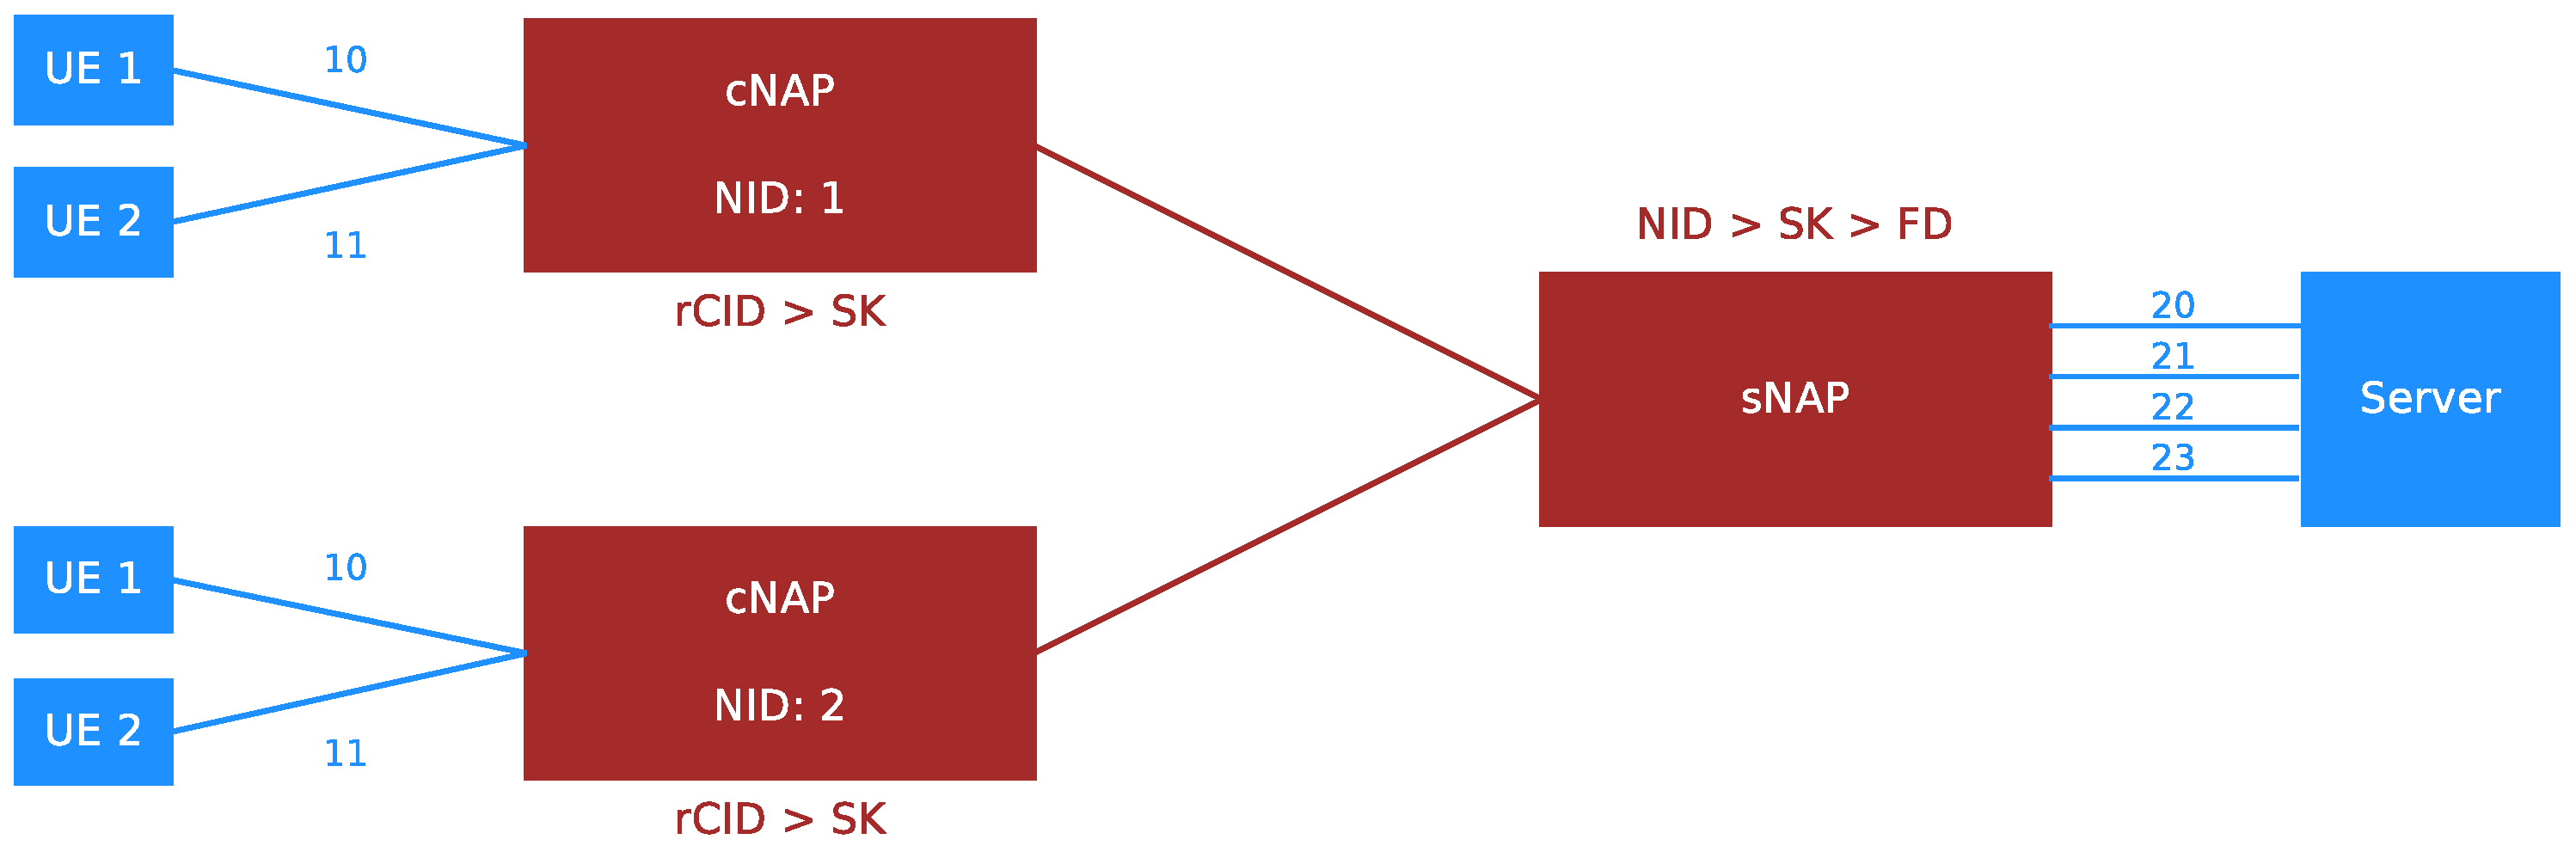
\includegraphics[width=1\linewidth]{eps/tcpSocketMappings}
\caption{Handling of TCP sockets across \aclp{NAP} an HTTP session}
\label{fig:TCP_Socket_Mappings}
\end{figure}

When the HTTP request is received by the \ac{sNAP} (\texttt{PUBLISHED\_DATA\_iSUB} in \texttt{icn.*}) the \ac{LTP} method \texttt{handle()} informs the callee if all segments have been received and therefore the received bytes (HTTP request) can be sent off to the server. At this stage \ac{LTP} also returned the used \ac{SK} so that the \ac{sNAP} can hand this information together with the \ac{NID} to the method \texttt{TcpClient::preparePacketToBeSent()} immediately followed by calling the functor \texttt{TcpClient::operator()()} to place the actual socket communication into a dedicated thread. Once this is done the respective thread looks up the private map \texttt{\_socketFds} which holds a mapping of \acp{NID} to remote socket \acp{FD} to local socket \acp{FD}, realised as an unordered \ac{STL} map within another \ac{STL} map (\texttt{u\_map<key, u\_map<key, value>>}). If a socket \ac{FD} is found it means that a socket has been already opened and it can be re-used. In that way \ac{TCP} socket re-use has been realised.

Table~\ref{tab:TCP_Socket_Mappings_sNAP_Request} depicts the mapping stored in \texttt{\_socketFds} from the exemplary scenario illustrated in Figure~\ref{fig:TCP_Socket_Mappings}. The \ac{NID} is used as the key for the outer map and the remote socket \ac{FD} as the key for the inner map (which is the value to the outer map's \ac{NID}). Consequently, the local socket \ac{FD} then is the value for the remote socket \ac{FD} map key.

\begin{table}[t]
	\centering
	\caption[TCP socket mappings across NAPs]{TCP socket mappings across \aclp{NAP} within private \texttt{\_socketFds} map}	\label{tab:TCP_Socket_Mappings_sNAP_Request}
\begin{tabular}{|c|c|c|}
	\hline \textbf{\ac{NID}} & \textbf{Remote Socket \ac{FD}} & \textbf{Local Socket \ac{FD}} \\ 
	\hline 1 & 10 & 20 \\ 
	\hline 1 & 11 & 21 \\ 
	\hline 2 & 10 & 22 \\ 
	\hline 2 & 11 & 23 \\ 
	\hline 
\end{tabular}
\end{table} 

A mutex, \texttt{\_socketFdsMutex}\footnote{This Boost mutex is realised as a pointer to the respective class, as Boost does not allow to share the private mutex member being shared among all threads.}, is then used whenever an operation is performed on \texttt{\_socketFds}, as the private members are shared among all threads created from the ICN handler class. So once a new HTTP request arrives at the \ac{sNAP} the \texttt{\_socketFds} map allows to look up if an existing socket \ac{FD} is known; if not, a new socket is created. This functionality is implemented in \texttt{TcpClient::\_tcpSocket()}. If the \ac{TCP} client in the \ac{sNAP} detects that the web server has shut down the \ac{TCP} session or the socket is simply nto readable anymore the local socket \ac{FD} is getting removed from \texttt{\_socketFds} map. If either the inner or the inner and the outer map are empty (no values left) they will be erased accordingly to keep the look-up time to find \ac{NID} or remote socket \ac{FD} keys to a bare minimum in the \ac{sNAP}.

When the \ac{HTTP} response issued by the web server is received at the \ac{sNAP} it is potentially sent out via co-incidential multicast which means that all \acp{cNAP} which are in the \ac{CMC} group will receive the response under the same randomly generated \ac{SK}. That is why \acp{cNAP} keep the relation of published \ac{HTTP} requests and their \ac{rCID} to the socket \acp{FD} which await the response. This is realised via the private member map \texttt{\_ipEndpointSessions} in the class \texttt{HTTP} which upon arrival of an \ac{HTTP} response at the \ac{cNAP} the received \ac{rCID} is used to retrieve the list of \acp{UE} awaiting this response.

%%%%%%%%%%%%%%%%%%%%%%%%%%%%%%%%%%%%%%%%%%%%%%%%%%%%%%%%%%%%%
% Section
%%%%%%%%%%%%%%%%%%%%%%%%%%%%%%%%%%%%%%%%%%%%%%%%%%%%%%%%%%%%%
\section{\acl{NAP} Packet Buffers}\label{sec:Code_NapPacketBuffers}
Another important implementation is the usage of packet buffers in order to accommodate for packet loss, enable packet reassembly and buffer packets to be published into the ICN network. In order to cover all the different buffers and implementation design choices to realise them this section is split into the following logical packet flows:

\begin{itemize}
	\item Packets arrive from an IP endpoint at a \ac{cNAP}
	\item Packets arrive at an \ac{sNAP} from the local \ac{ICN} core
	\item Packets arrive from IP endpoints at an \ac{sNAP}
	\item Packet arrive at a \ac{cNAP} from the local \ac{ICN} core
\end{itemize} 

The list above also reflects the logical flow of an IP communication (\ac{HTTP} in particular). When handling IP packets in the \ac{NAP} (using the IP handler) there is no difference whether the IP packet was issued by a server or by a client; in case this is an IP packet which carries \ac{HTTP} it does make a difference.

\subsection{Buffer Cleaners}
In order to not buffer packets infinitely in case no subscriber ever appears the \ac{NAP} has a dedicated buffer cleaner thread implemented which has access to both IP and \ac{HTTP} buffers via pointers to the actual maps and their corresponding mutexes to guarantee thread safe read and write actions. The IP and the HTTP buffer cleaners are initialised in the IP and HTTP namespace class constructor, respectively. As the C++ namespacing of the NAP (to allow class-based logging\footnote{See Section~\ref{sec:Introduction_Logging} for more details about this functionality}) does not allow to pass a reference to the IP and HTTP buffer and mutex the buffer constructors take void pointers only (see constructors in header files, \texttt{namespaces/buffercleaners/*.hh}) which are then casted back into their respective types (see constructor implementations in source files, \texttt{namespaces/buffercleaners/*.cc}).

A thread per \ac{ICN} namespace is opened in each namespace constructor which wakes up every $n$ seconds where $n$ is the value of the \ac{NAP} configuration variable \texttt{bufferCleanerInterval} (see Section~\ref{sec:Introduction_Var_BufferCleanerInterval}).

\subsection[IP Packets Issued by Endpoints towards cNAPs]{IP Packets Issued by Endpoints towards \aclp{cNAP}}
This sub-section describes the used packet buffers which are used when IP packets were issued by an IP endpoint which behaves as an IP client in this scenario. A graphical representation of the used buffers can be found in Figure~\ref{fig:packetBuffers-incomingIpPackets-cNap} with red boxes and arrows indicating IP traffic and golden boxes and arrows indicating \ac{HTTP} packet handling.

\begin{figure}
	\begin{center}
		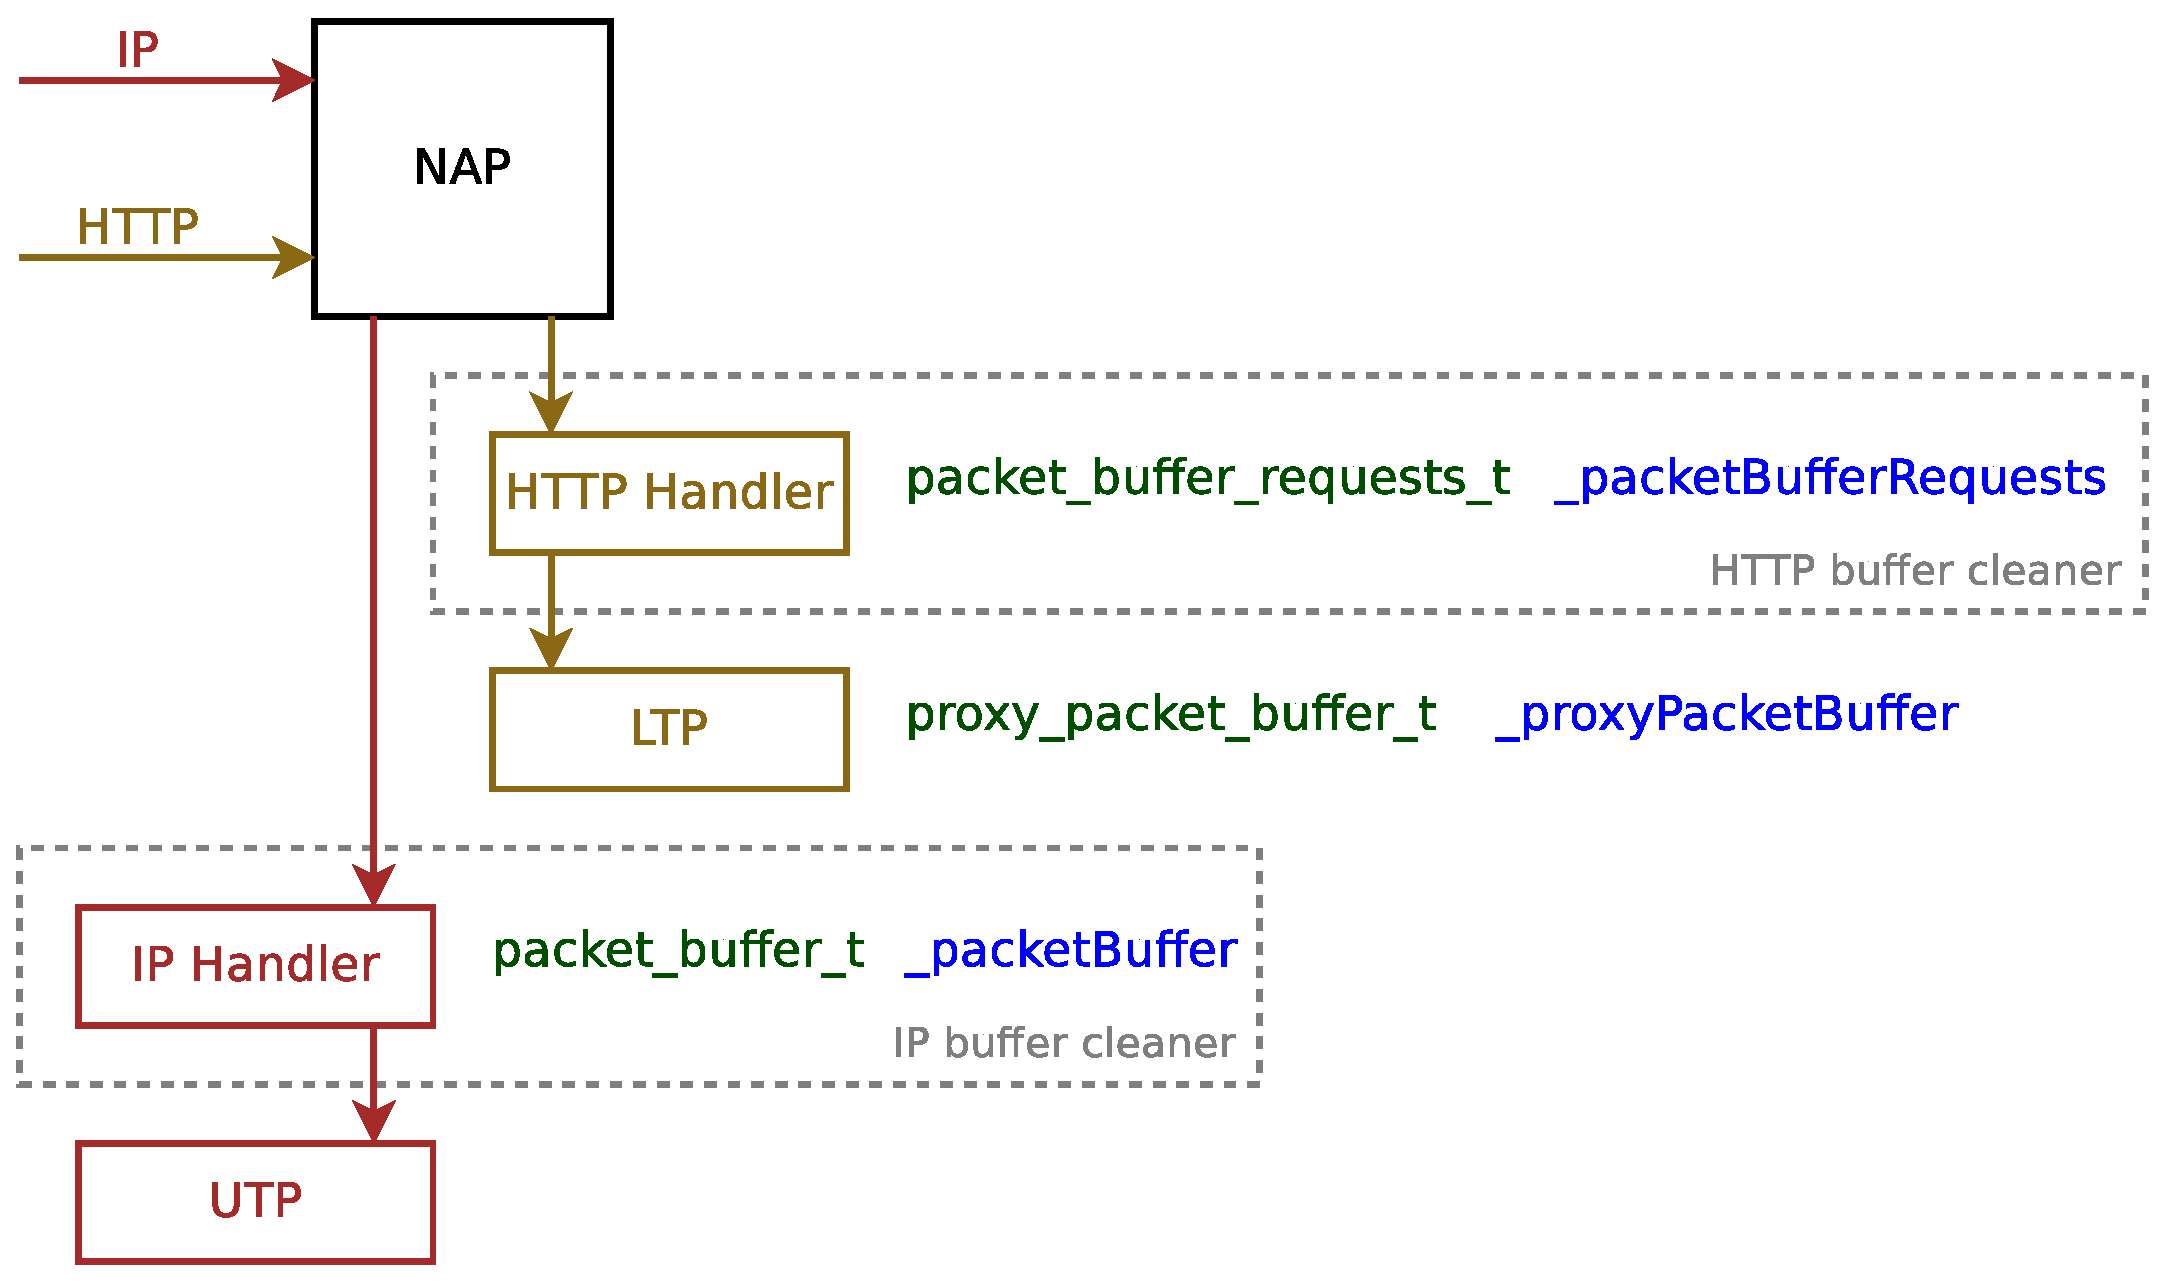
\includegraphics[width=0.8\textwidth]{eps/packetBuffersInTheNap-incomingIpPackets-cNap.eps}
		\caption{Packet buffers in the \acl{cNAP} for IP packets issued by endpoints}
		\label{fig:packetBuffers-incomingIpPackets-cNap}
	\end{center}
\end{figure}

\paragraph{IP}
For services other than HTTP (or any other future non-IP service) the IP handler is selected and the respective packet buffers to the left in Figure~\ref{fig:packetBuffers-incomingIpPackets-cNap} are used. The implementation of the IP handler defined in \texttt{namespaces/ip.hh} uses a predefined type \texttt{packet\_buffer\_t} which uses the hashed \ac{CID} as the map's unique key and a pair of the \ac{CID} of type \texttt{IcnId} and a packet description struct of type \texttt{packet\_t} as its values; both typedefs can be found in \texttt{namespaces/iptypedef.hh} and the \texttt{IcnId} class in \texttt{types/icnid.hh} (see Section~\ref{sec:Types_IcnId} on Page~\pageref{sec:Types_IcnId}). The buffer in the IP handler is solely used to buffer IP packets which could be published to the \ac{ICN} core at the time. Reason being the entire \ac{CID} needs to be published first to the \ac{RV} or the \ac{NAP} has not received a \texttt{START\_PUBLISH} notification for the \ac{CID} under which the IP packet needs to be published. If a \texttt{START\_PUBLISH} event arrives through the Blackadder API (see \texttt{icn.hh}) the \ac{ICN} handler has a reference to all namespaces (i.e. \texttt{\_namespaces}) which allows to look up the IP buffer for pending packets to be published via the method \texttt{Namespaces::publishFromBuffer} which switches based on the root scope into the particular namespace buffer (see \texttt{namespaces/namespace.cc}).

Any ready-to-be-published packet, either directly from the IP handler or through the buffer, is passed on to the \ac{UTP} implementation which simply publishes the packet following the methods and procedures described in Section~\ref{sec:Transport_UTP} on Page~\pageref{sec:Transport_UTP}.

\paragraph{HTTP}
Similar to IP, the HTTP namespace has several buffers which are frequently cleaned up in case the packets were not sent/published.
%%%%%%%%%%%%%%%%%%%%%%%%%%%%%%%%%%%%%%%%%%%%%%%%%%%%%%%%%%%%
% Section
%%%%%%%%%%%%%%%%%%%%%%%%%%%%%%%%%%%%%%%%%%%%%%%%%%%%%%%%%%%%%
\section{\acl{CMC} Group Formation}
Whenever the NAP maps an incoming packet to the HTTP-over-ICN name-space, the formation of multicast groups is realised at the \ac{sNAP} for the provisioning of HTTP responses to any \ac{cNAP} which awaits such message. The logical steps required are illustrated in a message sequence chart in Figure~\ref{fig:CmcGroupManagement}.

\begin{figure}
  \begin{center}
    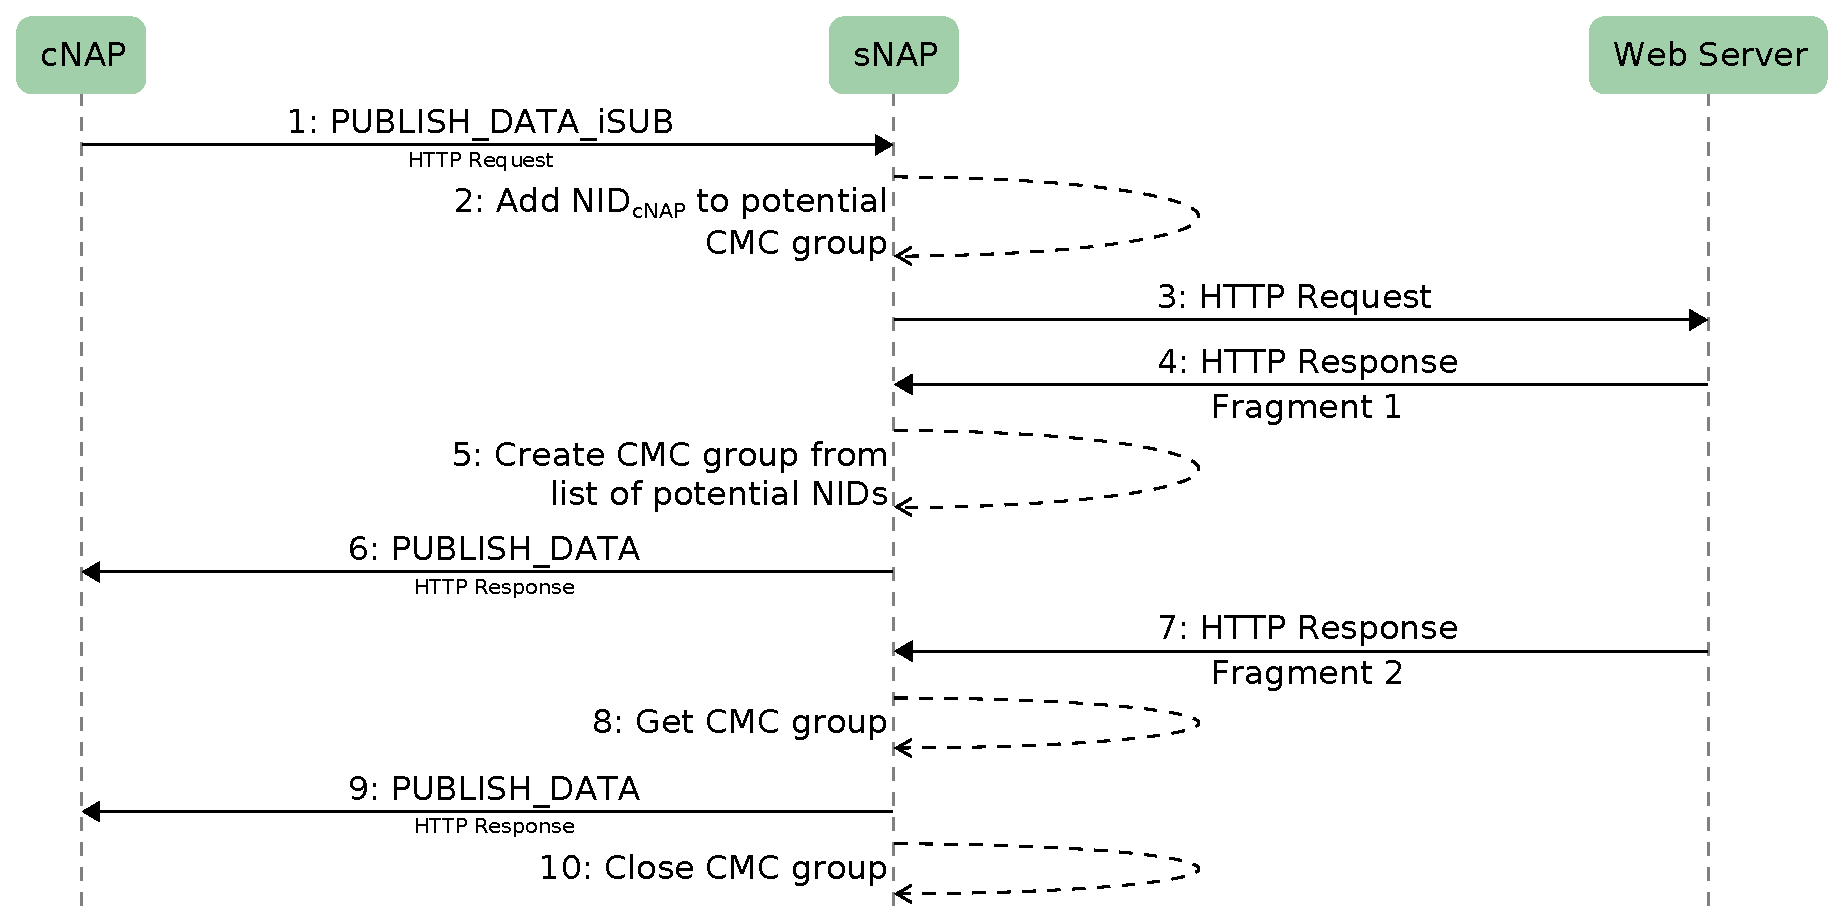
\includegraphics[width=\textwidth]{eps/cmcGroupManagement.eps}
    \caption{\acl{CMC} Group Formation at \acl{sNAP}}
    \label{fig:CmcGroupManagement}
  \end{center}
\end{figure}

\begin{enumerate}
	\item The \ac{cNAP} has published an HTTP request to an \ac{sNAP} which has subscribed to the respective \ac{FQDN}.
	\item Assuming there is no \ac{CMC} group for this particular \ac{URL}, the \ac{sNAP} creates a new potential \ac{CMC} group with the hashed \ac{URL} (\ac{rCID}) as the unique key and adds the \ac{cNAP}'s \ac{NID} to the list of \acp{NID} in this potential \ac{CMC} group.
	\item The \ac{sNAP} now delivers the HTTP request to the IP service endpoint via its transparent HTTP proxy (see Section~\ref{sec:Code_Transparent_HTTP_Proxy} for more information about the proxy). Furthermore, it stores a backwards mapping of socket file descriptor to \ac{rCID}.
	\item The IP service endpoint responds with the first (and maybe only) fragment of the entire HTTP response. The HTTP proxy receives this via the socket created in Step 3. 
	\item The \ac{sNAP} looks up the \ac{rCID} for this particular socket file descriptor and obtains the \ac{rCID}. With the \ac{rCID} the \ac{sNAP} finds all \acp{NID} awaiting the response in the potential \ac{CMC} group map. The \ac{sNAP} closes the group from allowing future \acp{cNAP} to become a member.
	\item The \ac{sNAP} publishes the HTTP response to the \ac{CMC} group of \acp{NID}.
	\item Assuming the HTTP response is made up of more than one fragment, the web server sends this to the \ac{sNAP} which still has a TCP opened via its transparent HTTP proxy. Using the mapping from Step 3 the \ac{sNAP} obtains the \ac{rCID} and looks up if a \ac{CMC} group is known which is awaiting this response.
	\item The \ac{sNAP} publishes the HTTP response to the group.
	\item The web server closes the socket which is dected in the HTTP proxy
	\item The \ac{sNAP} closes the \ac{LTP} session by sending an \ac{LTP}-CTRL-\ac{SE} message which must be confirmed by all \acp{cNAP}
	\item The \ac{sNAP} closes the \ac{CMC} group
\end{enumerate}
%%%%%%%%%%%%%%%%%%%%%%%%%%%%%%%%%%%%%%%%%%%%%%%%%%%%%%%%%%%%%
% Section
%%%%%%%%%%%%%%%%%%%%%%%%%%%%%%%%%%%%%%%%%%%%%%%%%%%%%%%%%%%%%
\section{Traffic Control}
The \ac{NAP} has received some prelimenary functionality to perform traffic control actions on to-be-published data packets; it is important to understand that this functional extension is solely influencing packets originated from an IP endpoint. Blackadder-related control plane packets sent by the NAP, e.g., scope publications or publication of information items, are not affected by this.

\subsection{Background}
The reason behind this particular functionality was mainly caused by functional testing purposes of \ac{LTP} (error control to be precise) in environments where the network does not cause any packet loss. Without any lost packet \ac{LTP}'s error control mechanism was hard to be tested and validated and using Linux's internal traffic control \cite{BertHuber} would simply affect every single packet traversing a particular interface, including Blackadder control plane traffic. As no control plane reliability existed (at least at the stage when \ac{LTP} was being tested), a \texttt{tc}-like module was written for the \ac{NAP} which simply acts on packets to be publish using the \texttt{publish\_data()} Blackadder primitive. As for \texttt{tc}, the respective traffic control module consists (theoretically) on the following filtering/traffic shaping mechanisms:

\begin{itemize}
  \item Shaping
  \item Scheduling
  \item Policing
  \item Dropping$^*$
\end{itemize}

However, at this stage only filtering/traffic shaping mechanisms marked with an ($^*$) have been realised.

\subsection{Implementation}
The corresponding implementation of all tc mechanisms are collated in a derived class \texttt{TrafficControl} in \texttt{trafficcontrol/trafficcontrol.hh}. \texttt{TrafficControl} is then made a public member of class \texttt{Lightweight} in \texttt{transport/lightweight.hh}. Thus, all implemented traffic control gets only applied to packets published via \ac{LTP} (for the time being).

In order to not break the code flow in the \ac{NAP} when it comes to manipulating the publication of data packets the realisation of traffic control is realised as followed: every time a packet has been prepared to be published (across the entire \ac{LTP} code in \texttt{transport/lightweight.cc}) the traffic control method \texttt{handle()} is called in an \texttt{if} statement. This method returns true if packet is supposed to be sent or false if not.

\subsubsection{Dropping}
The dropping of packets has been implemented as a binary decision within the class \texttt{Dropping}. When a packet is about to be published the respective \ac{LTP} method calls \texttt{TrafficControll::handle()} from where \texttt{Dropping:: dropPacket()} is called which has a boolean return. 

The \texttt{dropPacket()} method first checks if droppping was requested by the user when adjusting/writing the \ac{NAP} configuration file. This has been realised through the method \texttt{Configuration::tcRopRate()} (declared in \texttt{configuration.hh}) which returns \texttt{-1} if \texttt{tcDroppingRate} has not been set in the configuration file. If that has not been the case C's standard element function \texttt{rand()}, from \texttt{stdlib.h}, is being used together with the configured drop rate:

\begin{lstlisting}
rand() % _configuration.tcDropRate()
\end{lstlisting}

This essentially returns a value between \texttt{0} and $\text{tcDropRate} - 1$. If the outcome is \texttt{0} the method returns true (as in packet should be dropped); if the result is different from \texttt{0} the method returns false. The return value is directly returned to the place in \ac{LTP} where \texttt{TrafficControl::handle()} has been called.

\subsection{Configuration}
In order to enable this feature the following compilation flag \texttt{-DTRAFFIC\_CONTROL} must be set in the Makefile (\texttt{INC\_DIR}). 

\subsubsection{Dropping}
The dropping filter can be configured via the \ac{NAP} configuration file using the variable
\newline
\newline
\texttt{tcDroppingRate = <VALUE>}
\newline
\newline
This variable accepts unsigned integer values between 0 and 2$^{32}$ and represents the rate data packets will be dropped on average. For instance, if 100 is given to \texttt{tcDroppingRate} the NAP drops one in 100 to be published packets. Note, as \ac{LTP} has been designed and implemented for well managed networks it is not advisable to set the rate lower than 100. Experiments have shown that in this case the \ac{LTP} state machine of both publishing and subscribing endpoints gets out of sync.
\section{Monitoring via \acl{MOLY}}\label{sec:Code_MOLY}

%%%%%%%%%%%%%%%%%%%%%%%%%%%%%%%%%%%%%%%%%%%%%%%%%%%%%%%%%%%%%
% Bibliography
%%%%%%%%%%%%%%%%%%%%%%%%%%%%%%%%%%%%%%%%%%%%%%%%%%%%%%%%%%%%%
\bibliographystyle{plain}
\bibliography{nap.bib} 
\end{document}
